\documentclass[12pt]{article}
\usepackage{amsmath,amssymb}
\usepackage{amsthm}
\usepackage{graphicx}
\usepackage[shortlabels]{enumitem}
\setlength{\hoffset}{-0.33in}
\setlength{\voffset}{-1in}
\setlength{\textwidth}{6in}
\setlength{\textheight}{9in}

\renewcommand{\i}{\infty}

\newcommand{\cA}{{\mathcal A}}
\newcommand{\cB}{{\mathcal B}}
\newcommand{\cC}{{\mathcal C}}
\newcommand{\cD}{{\mathcal D}}
\newcommand{\cE}{{\mathcal E}}
\newcommand{\cF}{{\mathcal F}}
\newcommand{\cH}{{\mathcal H}}
\newcommand{\cI}{{\mathcal I}}
\newcommand{\cK}{{\mathcal K}}
\newcommand{\cL}{{\mathcal L}}
\newcommand{\cM}{{\mathcal M}}
\newcommand{\cN}{{\mathcal N}}
\newcommand{\cO}{{\mathcal O}}
\newcommand{\cP}{{\mathcal P}}
\newcommand{\cR}{{\mathcal R}}
\newcommand{\cS}{{\mathcal S}}
\newcommand{\cT}{{\mathcal T}}
\newcommand{\cU}{{\mathcal U}}
\newcommand{\cV}{{\mathcal V}}
\newcommand{\cW}{{\mathcal W}}
\newcommand{\cY}{{\mathcal Y}}

% bold letters
\newcommand{\bZ}{{\mathbb Z}}
\newcommand{\bR}{{\mathbb R}}
\newcommand{\bC}{{\mathbb C}}
\newcommand{\bT}{{\mathbb T}}
\newcommand{\bN}{{\mathbb N}}
\newcommand{\bQ}{{\mathbb Q}}

\newcommand{\bE}{{\boldsymbol E}}

\theoremstyle{definition}
\newtheorem{definition}{Definition}
\newtheorem{theorem}{Theorem}
\newtheorem{cor}{Corollary}
\newtheorem{lemma}{Lemma}
\newtheorem{eg}{Example}


\begin{document}

\graphicspath{ {images/} }
\pagestyle{empty}

\noindent
\textbf{Proposition:} Let $M\subset \bR^3$ be a compact surface and  $f:M\rightarrow \bR$ a morse function on $M$. Define $A := \#$ critical points (of f) with index 0, $B:= \#$ critical points with index 1, and $C:=\#$ critical points with index 2. Then, the Euler characteristic $\chi_M$ of $M$ is given by $\chi_M = A-B+C$. \\

We start by giving a list of definitions and proving some useful lemmas. 

\begin{definition}[Simplicial 1,2-Complex]
      A \textbf{simplicial 1-complex} is a topological space consisting of points and line segments, identified by verticies and along edges. 

      A \textbf{simplicial 2-complex} is a topological space consisting of points, line segments, and triangles identified along verticies and edges. 
\end{definition}

\textbf{Examples and Non-examples}
\begin{eg}
      The following are all simplicial 2-complexes:
      \begin{enumerate}
            \item A point
            \item A line segment between two points
            \item A triangle consisting of three line segments connecting three points
      \end{enumerate}
\end{eg}

\begin{eg}
      The following are \textbf{NOT} simplicial 2-complexes
      \begin{enumerate}
            \item 
      \end{enumerate}
\end{eg}


\begin{definition}[Euler Characteristic]
      The \textbf{Euler characteristic} $\chi$ of a simplicial 2-complex is given by the formula 
      \begin{center}
            $\chi = V-E + F$
      \end{center}
      where $V$ is the number of verticies, $E$ is the number of edges, and $F$ the number of triangles (faces). 
      
\end{definition}

We will be using the following two theorems without including proofs.

\begin{theorem}
      If $P_1, P_2$ are homeomorphic simplicial 2-complexes, then $\chi(P_1) = \chi(P_2)$
\end{theorem}

\begin{theorem}
      Every compact n-manifold $M$ is homeomorphic to a simplicial n-complex $P$. We can define $\chi(M) := \chi(P)$. 
\end{theorem}

\begin{theorem}
      Let $P,Q$ be two disjoint simplicial n-complexes, then we have that 
      \begin{center}
            $\chi(P\sqcup Q) = \chi(P) + \chi(Q)$. 
      \end{center}
\end{theorem}

\begin{proof}
      Let $\{V_1,E_1,F_1\} \subset \bN^3$ be the number of verticies, edges, and faces of $P$, $\{V_2,E_2,F_2\}$ that of $Q$. Then, since $Q \cap P = \emptyset$, we have that the total number of verticies of $Q\sqcup P$ is $V_1+V_2$, and the same goes for $\#$ edges and faces. Thus we get $\chi(P\sqcup Q) = V_1 +V_2 -(E_1+E_2)+F_1+F_2 = V_1-E_1+F_1 + V_2-E_2+F_2 = \chi(P) +\chi(Q)$. 
\end{proof}

\noindent
In the context of Morse theory on surfaces, we can look for simplicial 2-complexes homeomorphic to 0,1,2-handles and their ``attachment boundaries'' in order to extract information about their Euler characteristics. 

\begin{enumerate}
      \item \textbf{0-Handle}\\
            A 0-handle $H_0$ is homeomorphic to the 2-disk, $H_0 \cong D^2 \times D^0$, with attachment boundary $\partial_\cA H_0 \cong \partial D^2 \times D^0 \cong S^1$. The 2-disk is homeomorphic to a (filled) triangle, so $\chi(H_0) = 3 - 3 + 1 = 1$. Similarly, $S^1$ is homeomorphic to three verticies connected by 3 edges, ie. the perimeter of a triangle, so $\chi(\partial_\cA H_0) = 3-3+0 = 0$. 
            \begin{center}
                  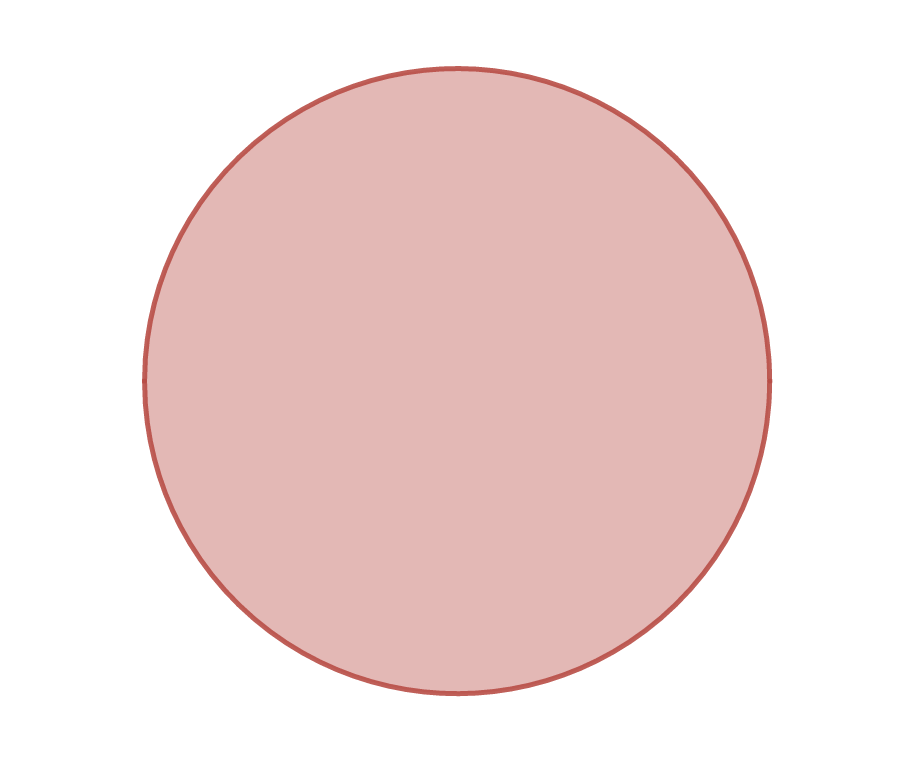
\includegraphics[scale=0.5]{H_0.png} \\
                  $H_0 \cong D^2$

                  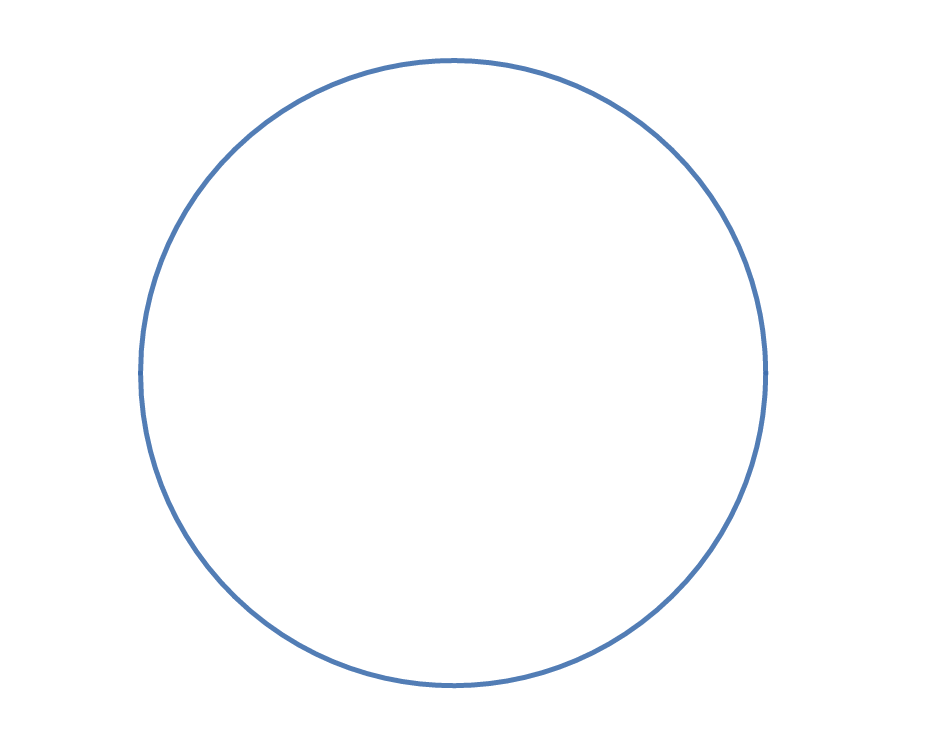
\includegraphics[scale = 0.5]{D H_0.png}\\
                  $\partial_\cA H_0 \cong S^1$
                  
            \end{center}
      \item \textbf{1-Handle}\\
            A 1-handle $H_1$ is homeomorphic to the cartesian product of two intervals, $H_1 \cong D^1\times D^1$ with attachment boundary $\partial_\cA H_1 \cong \partial D^1 \times D^1 \cong D^1 \sqcup D^1$. $H_1$ is also homeomorphic to the 2-disk, but another way to determine its Euler characteristic is by considering it as two (congruent, equilateral) triangles with one coincident edge. This gives $\chi(H_1) = 4 - 5+ 2 = 1$. The attachment boundary $\partial H_1$ is just given by two disjoint sets of two verticies and one edge connecting them, giving us $\chi(\partial_\cA H_1) = 4 - 2 + 0 = 2$. 
            \begin{center}
                  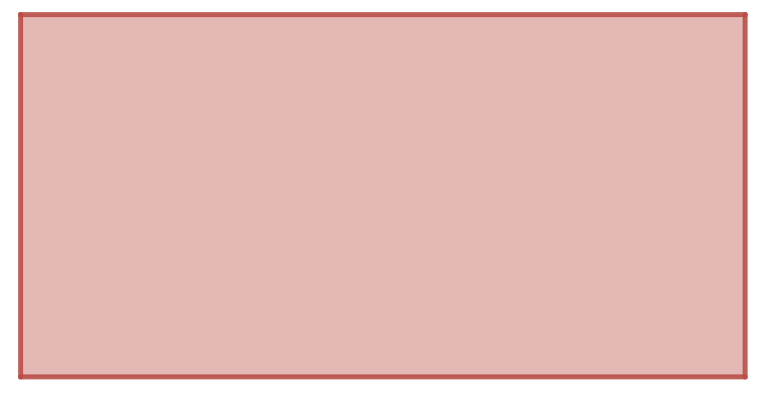
\includegraphics[scale=0.5]{H_1.png} \\
                  $H_1 \cong D^1\times D^1$

                  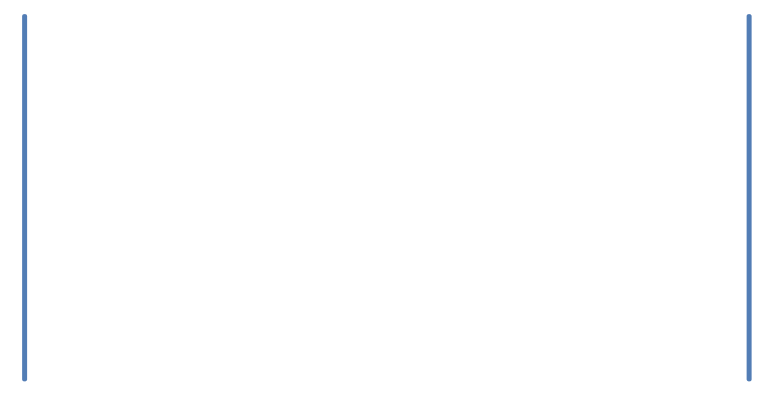
\includegraphics[scale = 0.5]{D H_1.png}\\
                  $\partial_\cA H_1 \cong D^1 \sqcup D^1$
            \end{center}
      \item \textbf{2-Handle}\\
            A 2-handle $H_2$ is homeomorphic to the 2-disk, $H_2 \cong D^0 \times D^2 \cong D^2$, with attachment boundary $\partial_\cA H_2 \cong S^1$. The 2-disk is homeomorphic to a (filled) triangle, so $\chi(H_0) = 3 - 3 + 1 = 1$. Similarly, $S^1$ is homeomorphic to three verticies connected by 3 edges, ie. the perimeter of a triangle, so $\chi(\partial_\cA H_0) = 3-3+0 = 0$. 
            \begin{center}
                  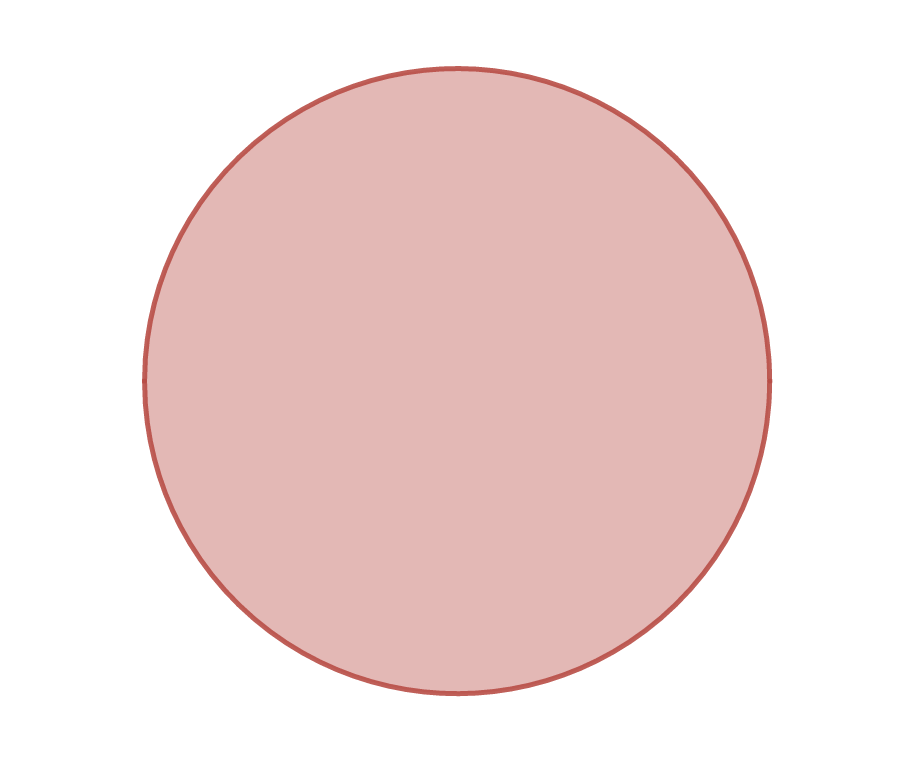
\includegraphics[scale=0.5]{H_0.png} \\
                  $H_2 \cong D^2$

                  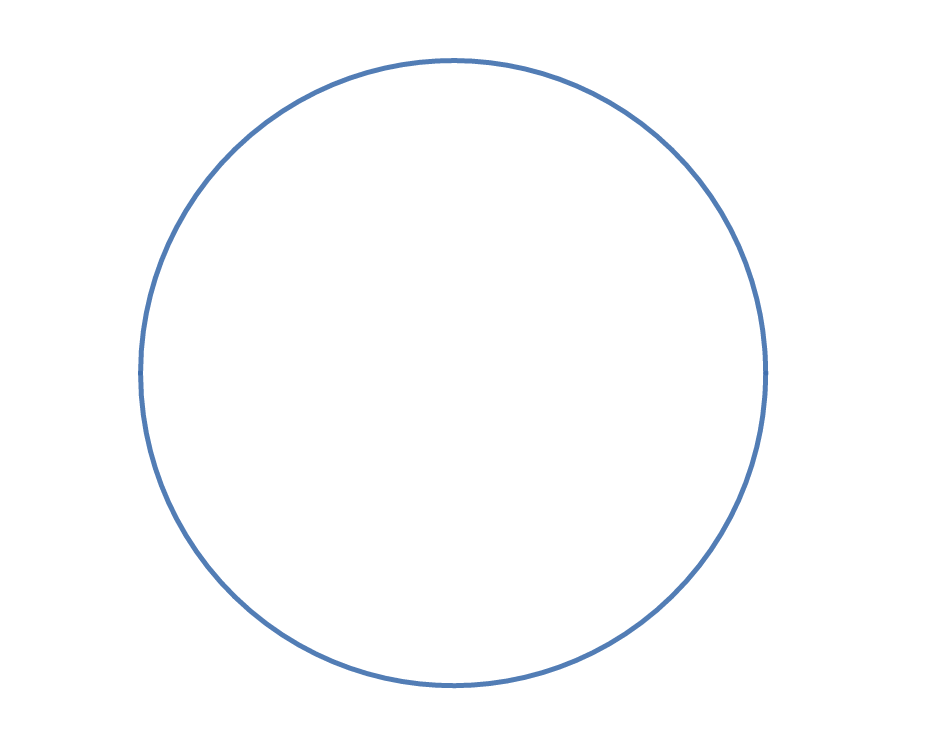
\includegraphics[scale = 0.5]{D H_0.png}\\
                  $\partial_\cA H_2 \cong S^1$
            
            \end{center}
\end{enumerate}

Now we can give the proof of the main result:
\begin{proof}
      Let $M \subset \bR^3$ be a compact manifold which exhibits a Morse function $f:M \rightarrow \bR$. Let $\{i_1,i_2,...,i_n\}\in \{0,1,2\}^n$ denote the Morse indicies of the $n$ (non-degenerate) critical points $\{p_1,p_2,...,p_n\}$ of $f$. By the handle decomposition theorem, we know that $M$ is homeomorphic to the union of $A$ 0-handles, $B$ 1-handles, and $C$ 2-handles, where $A = \# \{i_j : i_j = 0\}, B = \# \{i_j : i_j = 1\}, C= \# \{i_j: i_j = 2\}$. To prove our desired result, we will split into cases of observing what happens to the Euler characteristic upon attaching a 0,1, or 2-handle. In each of the following cases, we will let $M_{p} = \{x \in M: f(x)\leq f(p)\}$, i.e. the sublevel set of $M$ at $p$. Note that the boundary $\partial M_{p} = \{x \in M : f(x) = f(p)\}$. 
      
      \begin{enumerate}
            \item $i_j = 0$\\
            In the case that our morse index is 0, we are simply taking the disjoint union $M_{p_{i_j}} \sqcup H_0$, so we can use our additivity property to get that $\chi(M \sqcup H_0) = \chi(M) + \chi(H_0) = \chi(M) + 1$. 

            \item $i_j = 1$\\
            Attaching a 1 handle is slightly more complicated. First, $M_{p_{i_j}}$ is homeomorphic to some simplicial 2-complex $\cS_M$ with $V_M$ verticies, $E_M$ edges, and $F_M$ faces. Furthermore $\partial M_{p_{i_j}}$ is homeomorphic to some simplicial 1-complex $\cS_j$ with $V_j$ verticies and $E_j$ edges, where $\cS_j \subseteq \cS_M$. We claim that we can assume that there are two distinct edges $E_1, E_2$ such that their endpoints (verticies called, say $V_1, V_1'$ and $V_2,V_2'$) are also distinct. We are free to assume this since the simplicial complex $\cS_j'$ created by adding verticies at the midpoints of each edge and ``splitting'' the original edge into two edges is homeomorphic $\cS_j$. 
            \begin{center}
                  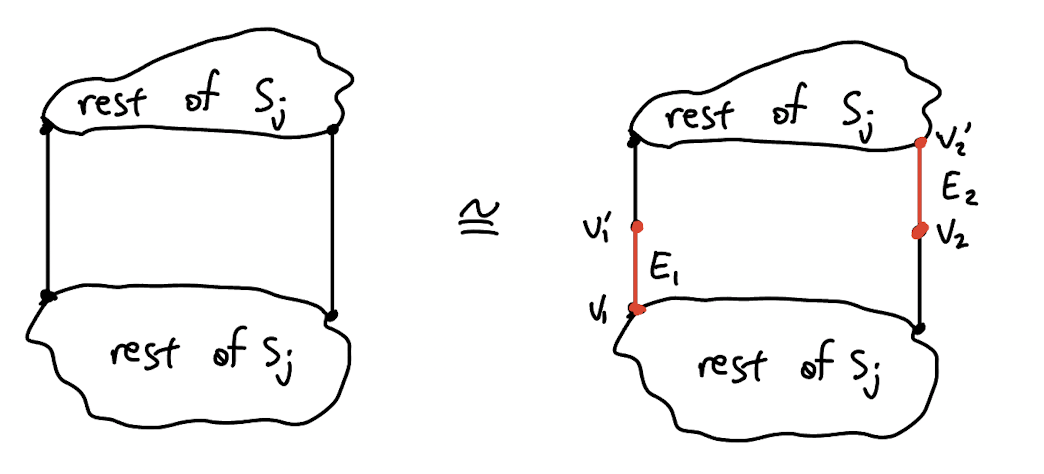
\includegraphics[scale = 0.7]{sim.png}
            \end{center}
            Now that we have a subset of $\cS_j$ which is homeomorphic to the attachment boundary $\partial_\cA H_1$, we can attach the handle to the boundary by identifying the respective edges and verticies. Concretely, our 1-handle $H_1$ is homeomorphic to a simplicial 2-complex with $V_H = 4, E_H = 5, F_H = 2$ with attachment boundary $\partial_\cA H_1$ homeomorphic to a simplicial 1-complex with $V_\partial = 4, E_\partial = 2$. Upon attaching, we identify the $V_\partial$ with $\{V_1,V_1',V_2,V_2'\}$ and $E_\partial$ with $\{E_1,E_2\}$ and we can recount the total number of verticies, edges, and faces to get the resulting Euler characteristic. Clearly, the number of faces is just the sum of the two parts, since we don't identify any faces, i.e. $F_{M\cup H_1} = F_M + F_H = F_M + 2$. Next, since we are now identifying 4 verticies of $H_1$ with those on $S_j$, we get that $V_{M\cup H_1} = V_M + V_H - 4 = V_M + 4 - 4 = V_M$ to account for double counting. Finally, we get something similar for the number of edges, namely $E_{M\cup H_1} = E_M + E_H - 2 = E_M + 5 - 2 = E_M + 3$. To get the Euler characteristic, we apply our formula to get $\chi(M \cup H_1) = V_M - E_M - 3 + F_M + 2 = V_M - E_M+ F_M -1 = \chi(M)-1$
            

            \item $i_j = 2$\\
            In order to even attach a 2-handle to $M_{p_{i_j}}$, we necessarily require that there be a connected component of $\partial M_{p_{i_j}}$ which is homeomorphic to $S^1$. Because the attachment boundary of $H_2$ is exacly $S^1$ (which is homeomorphic to a triangle), we get that $V_{M\cup H_2} = V_M + V_H - V_H = V_M$, since all verticies of $H_2$ are on its boundary. A similar statement holds for the edges of $H_2$, so we get $E_{M\cup H_2} = E_M + E_H - E_H = E_M$. As for faces, since we are only identifying the edges and verticies as subsets of the simplicial 2-complexes, the resulting number of faces is just the sum of the two parts, $F_{M\cup H_2} = F_M + F_H = F_M + 1$. Counting, we get $\chi(M\cup H_2) = V_M -E_M + F_M +1 = \chi(M) + 1$. 
      \end{enumerate}

      From the above results, we see that we add 1 to our Euler characteristic everytime we attach a 0 or 2-handle, and subtract 1 everytime we attach a 1-handle, so 
      \begin{center}
            $\chi(M) = A-B+C$. 
      \end{center}
\end{proof}



% \textbf{Proof Outline}
% \begin{enumerate}
%       \item Definition of Euler Characteristic 
%       \begin{enumerate}
%             \item $\chi = V-E+F$ 
%             \item Euler characteristic of surfaces
%       \end{enumerate}
%       \item Existence of Triangulation/Polygonal Decomp of compact surfaces
%       \item Change in $\chi$ by attaching 0,1,2-handle
%       \begin{enumerate}
%             \item For a 0 handle, we add 1 to $\chi$ since we are adding a ``triangle'' (up to homeomorphism)
%             \item For a 1 handle, we subtract 1 to $\chi$ since we are essentially adding 2 edges and 1 face without changing verticies
%             \item For a 2 handle, we add 1 to $\chi$ since we are adding 1 face without changing any edges or verticies
%       \end{enumerate}
% \end{enumerate}

\end{document}